
% ============================================================
%  Presentation: Optimization Action Analyzer
%  Companion Beamer deck to the graduation-book chapter.
%  Compile with pdflatex (or lualatex/xelatex).
% ============================================================
\documentclass[aspectratio=169]{beamer}

\usetheme{Madrid}
\usecolortheme{beaver}

\usepackage[utf8]{inputenc}
\usepackage{graphicx}
\usepackage{booktabs}
\usepackage{tikz}
\usetikzlibrary{arrows.meta, positioning, shapes.geometric}

% ── Path to screenshots ─────────────────────────────────────
\graphicspath{{../figures/chapter06/}}

\title[Optimization Action Analyzer]{Optimization Action Analyzer}
\subtitle{Version-Controlled Telecom KPI Impact Analysis}
\author{}
\institute{}
\date{}

\begin{document}

% ══════════════════════════════════════════════════════════
\begin{frame}
    \titlepage
\end{frame}

% ══════════════════════════════════════════════════════════
\section{Introduction}

\begin{frame}{The Problem}
    \begin{quote}
        \emph{``Did the change we just made actually improve the network,
        and by how much?''}
    \end{quote}
    \vspace{0.5em}
    \begin{itemize}
        \item RAN optimization teams push configuration changes constantly
              (antenna tilt, TX power, handover parameters, carrier
              aggregation, \dots)
        \item Impact assessment requires knowing \textbf{what} changed,
              \textbf{when}, and comparing against a \textbf{fair
              baseline}
        \item Traditionally done manually, in spreadsheets --- slow and
              error-prone
    \end{itemize}
\end{frame}

\begin{frame}{Motivation}
    \begin{itemize}
        \item No single source of truth for ``what changed''
        \item Naive before/after comparisons ignore weekly seasonality
        \item Overlapping changes confound results
        \item Manual, non-repeatable analysis
    \end{itemize}
    \vspace{0.5em}
    \begin{block}{Solution}
        Combine a \textbf{version-controlled configuration database
        (Dolt)} with a \textbf{weekday-matched statistical comparison
        engine} and an \textbf{interactive visualization layer}.
    \end{block}
\end{frame}

% ══════════════════════════════════════════════════════════
\section{System Architecture}

\begin{frame}{High-level Module Architecture}
    \centering
    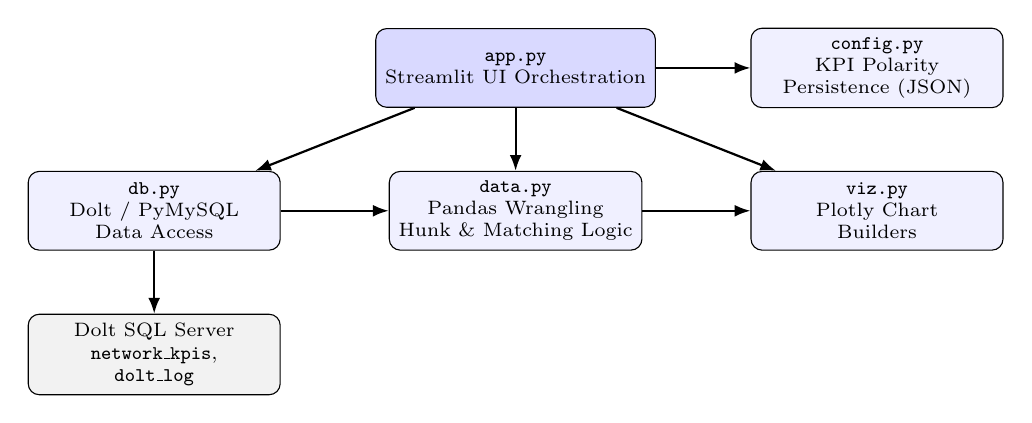
\begin{tikzpicture}[
        node distance=8mm and 12mm,
        box/.style={draw, rounded corners, minimum width=3.2cm,
                     minimum height=1.0cm, align=center, font=\scriptsize,
                     fill=blue!6},
        arrow/.style={-{Latex[length=2mm]}, thick}
    ]
        \node[box, fill=blue!15] (app) {\texttt{app.py}\\Streamlit UI Orchestration};
        \node[box, below left=of app] (db) {\texttt{db.py}\\Dolt / PyMySQL\\Data Access};
        \node[box, below=of app] (data) {\texttt{data.py}\\Pandas Wrangling\\Hunk \& Matching Logic};
        \node[box, below right=of app] (viz) {\texttt{viz.py}\\Plotly Chart\\Builders};
        \node[box, right=of app] (config) {\texttt{config.py}\\KPI Polarity\\Persistence (JSON)};
        \node[box, below=of db, fill=gray!10] (dolt) {Dolt SQL Server\\\texttt{network\_kpis},\\\texttt{dolt\_log}};

        \draw[arrow] (app) -- (db);
        \draw[arrow] (app) -- (data);
        \draw[arrow] (app) -- (viz);
        \draw[arrow] (app) -- (config);
        \draw[arrow] (db) -- (dolt);
        \draw[arrow] (db) -- (data);
        \draw[arrow] (data) -- (viz);
    \end{tikzpicture}

    \footnotesize High-level module architecture of the Optimization
    Action Analyzer. The Streamlit application (\texttt{app.py})
    orchestrates calls into four independent layers: database access,
    data wrangling, visualization, and configuration persistence.
\end{frame}

\begin{frame}{Module Responsibilities}
    \small
    \begin{tabular}{@{}p{2.2cm}p{8.8cm}@{}}
        \toprule
        \textbf{Module} & \textbf{Responsibility} \\
        \midrule
        \texttt{db.py}     & Dolt connection, KPI schema discovery, commit
                              log \& diff queries, KPI time-series fetch \\
        \texttt{data.py}   & Action Hunk grouping, rolling evaluation
                              window, weekday-matched Before/After
                              profiles \\
        \texttt{viz.py}    & Plotly figures: timeline, trend, delta bars,
                              summary table \\
        \texttt{config.py} & Persists KPI optimization polarity to
                              \texttt{kpi\_config.json} \\
        \texttt{app.py}    & Streamlit front-end wiring everything
                              together \\
        \bottomrule
    \end{tabular}
\end{frame}

% ══════════════════════════════════════════════════════════
\section{Data Model and Sources}

\begin{frame}{Data Sources}
    Served through a \textbf{Dolt} SQL server (version-controlled,
    Git-like relational database) via PyMySQL:
    \begin{enumerate}
        \item \textbf{\texttt{network\_kpis}} --- time-series KPI table
              (15-min granularity): throughput, drop rate, RACH success,
              CQI, BLER, latency, PRB utilization, handover success, SINR
        \item \textbf{\texttt{dolt\_log}} --- Dolt's built-in commit
              history: commit hash, committer, e-mail, timestamp, message
    \end{enumerate}
    \vspace{0.5em}
    \begin{alertblock}{Key idea}
        Dolt's own version history \emph{is} the action log --- no
        separate change-management system required.
    \end{alertblock}
\end{frame}

% ══════════════════════════════════════════════════════════
\section{Core Algorithms}

\begin{frame}{Action Hunks}
    \begin{itemize}
        \item Commits sharing the same calendar date are grouped into a
              single \emph{Action Hunk}
        \item \texttt{build\_action\_hunks()} produces one selectable
              unit of change per optimization event
        \item Label example: \texttt{"2024-06-10 (Mon) · 3 commits"}
    \end{itemize}
\end{frame}

\begin{frame}{Rolling Evaluation Window}
    \texttt{resolve\_eval\_window()} determines the ``After'' period:
    \begin{itemize}
        \item Starts on the hunk's date
        \item Ends at \emph{today} or the day before the \emph{next}
              hunk --- whichever is earlier
        \item \textbf{``Ignore Next Action Hunk''} toggle overrides the
              cap
    \end{itemize}
\end{frame}

\begin{frame}{Weekday-Matched Baseline Construction}
    \texttt{collect\_matching\_weekdays()}:
    \begin{enumerate}
        \item Match each After-window date to the same weekday exactly
              \textbf{7 days earlier}
        \item Average KPI values across all matching dates, by
              minute-of-day
        \item Align Before/After profiles to a common minute-of-day
              index
    \end{enumerate}
    \vspace{0.3em}
    \small \texttt{collect\_individual\_days()} preserves the same
    matching logic without averaging, grouped by weekday.
\end{frame}

\begin{frame}{Optimization Polarity}
    \begin{itemize}
        \item Each KPI is either \texttt{"higher"} or \texttt{"lower"}
              is better
        \item Inferred automatically from keywords (\texttt{drop},
              \texttt{error}, \texttt{latency}, \texttt{bler},
              \texttt{retry} $\Rightarrow$ lower is better)
        \item Editable in the sidebar, persisted to
              \texttt{kpi\_config.json}
        \item Drives colour-coding across the delta chart and summary
              table
    \end{itemize}
\end{frame}

% ══════════════════════════════════════════════════════════
\section{Visualization Layer}

\begin{frame}{Action Hunk Distribution --- hover for commit details}
    \centering
    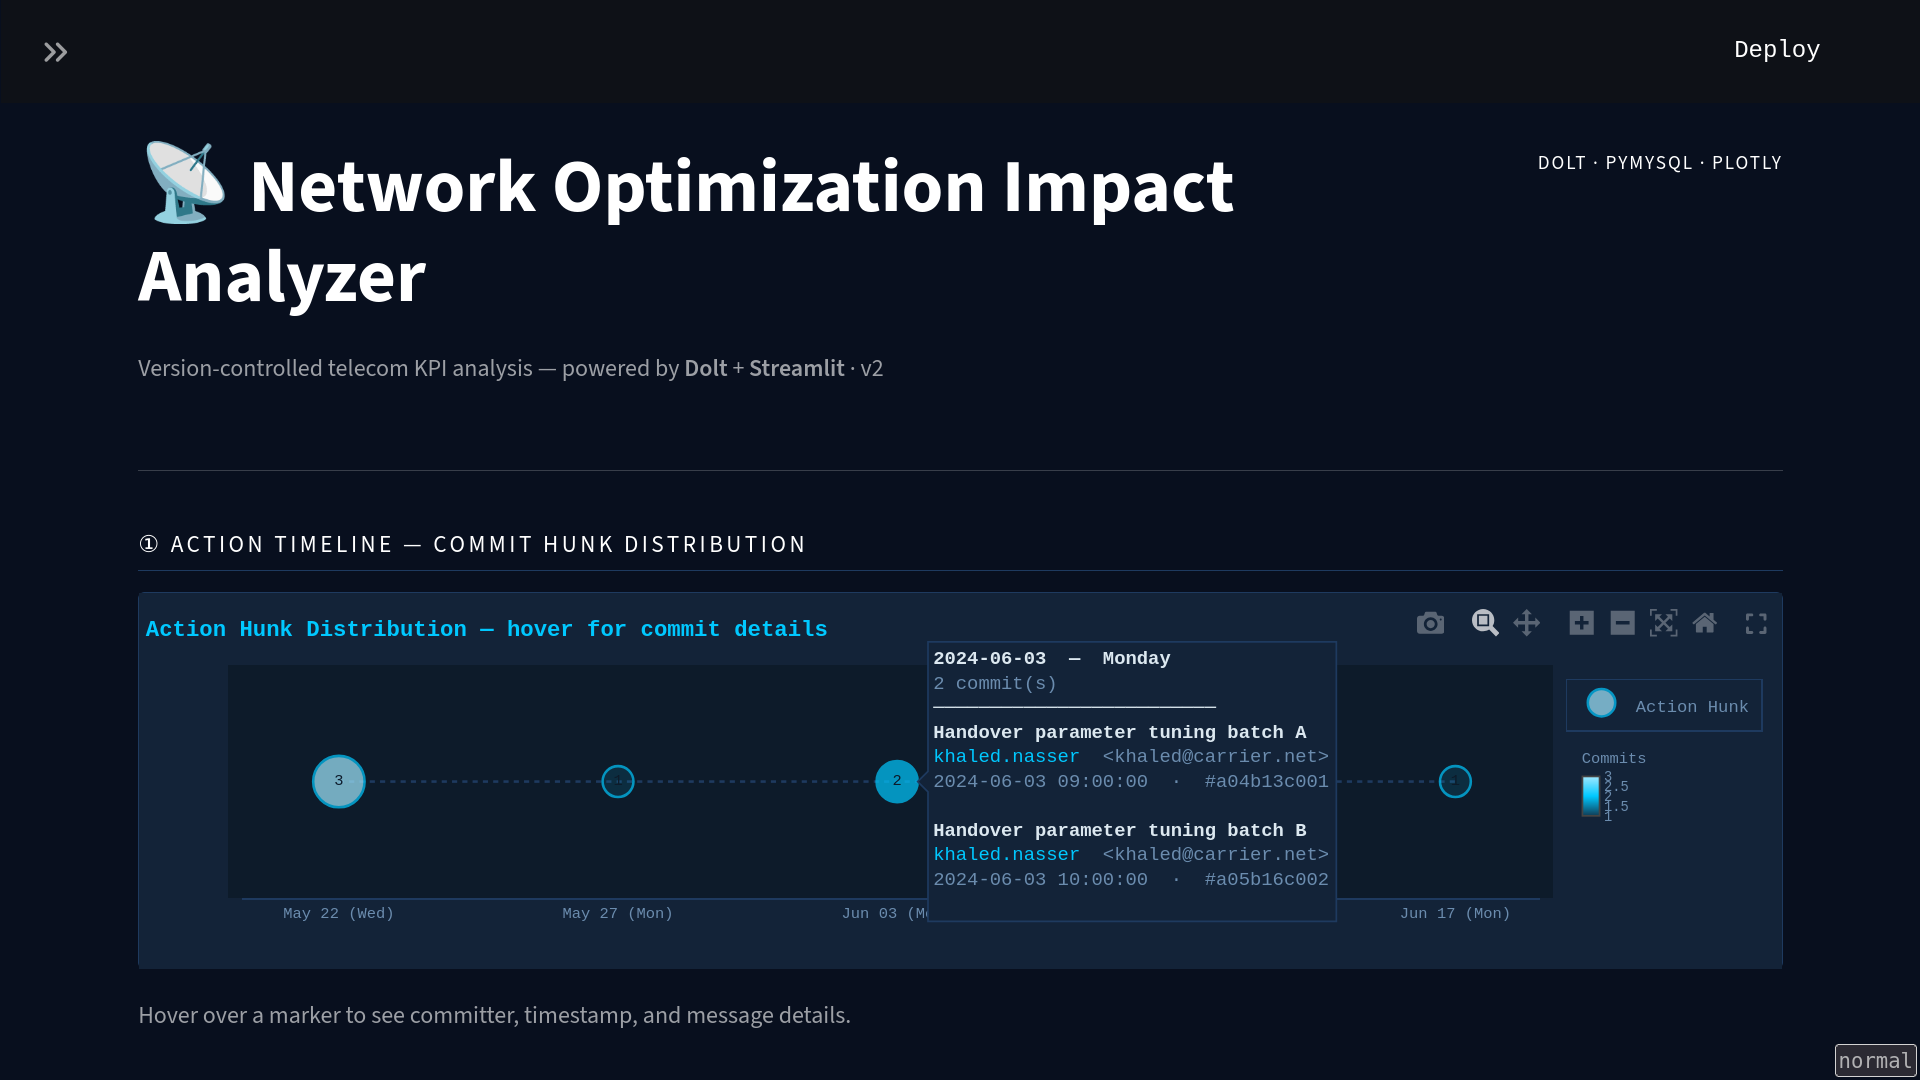
\includegraphics[width=0.85\textwidth]{action_timeline.png}
\end{frame}

\begin{frame}{KPI Trend --- Before vs. After}
    \centering
    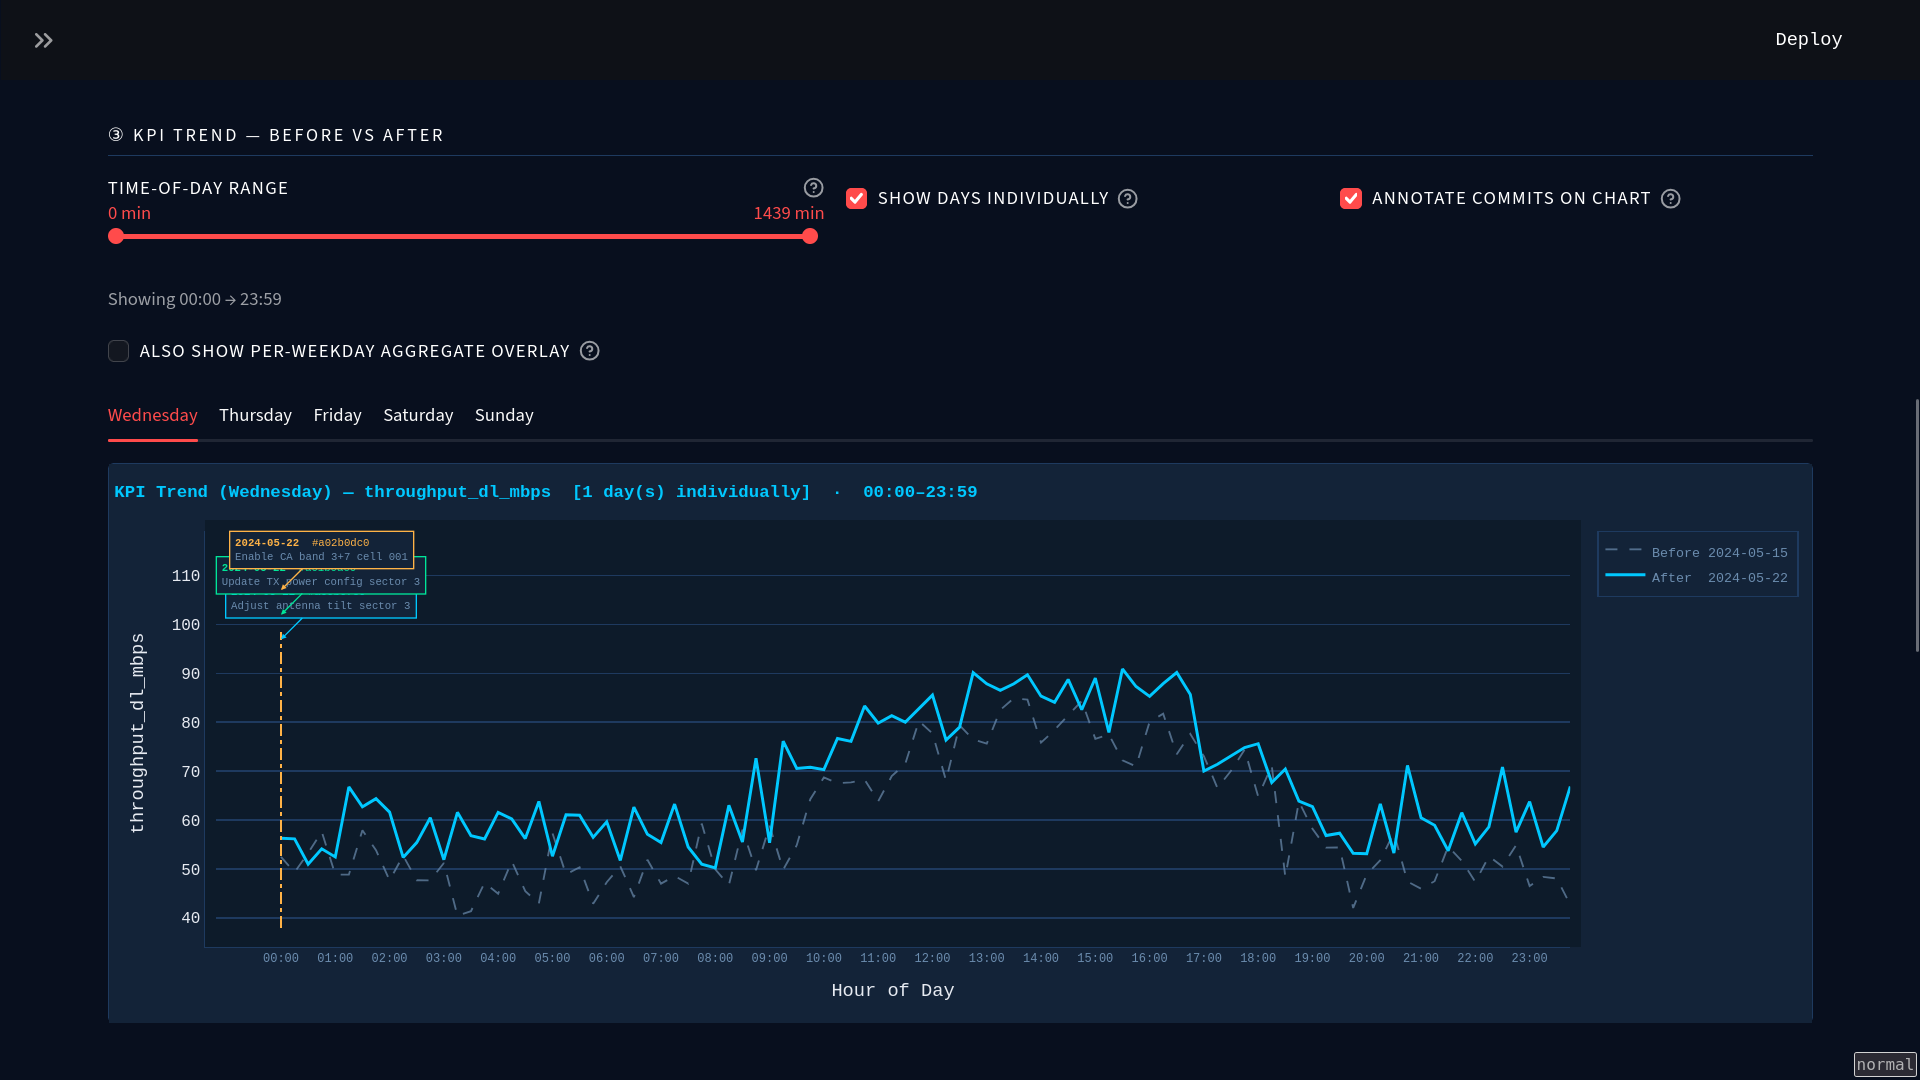
\includegraphics[width=0.85\textwidth]{kpi_trend.png}
\end{frame}

\begin{frame}{Interval Delta (After $-$ Before)}
    \centering
    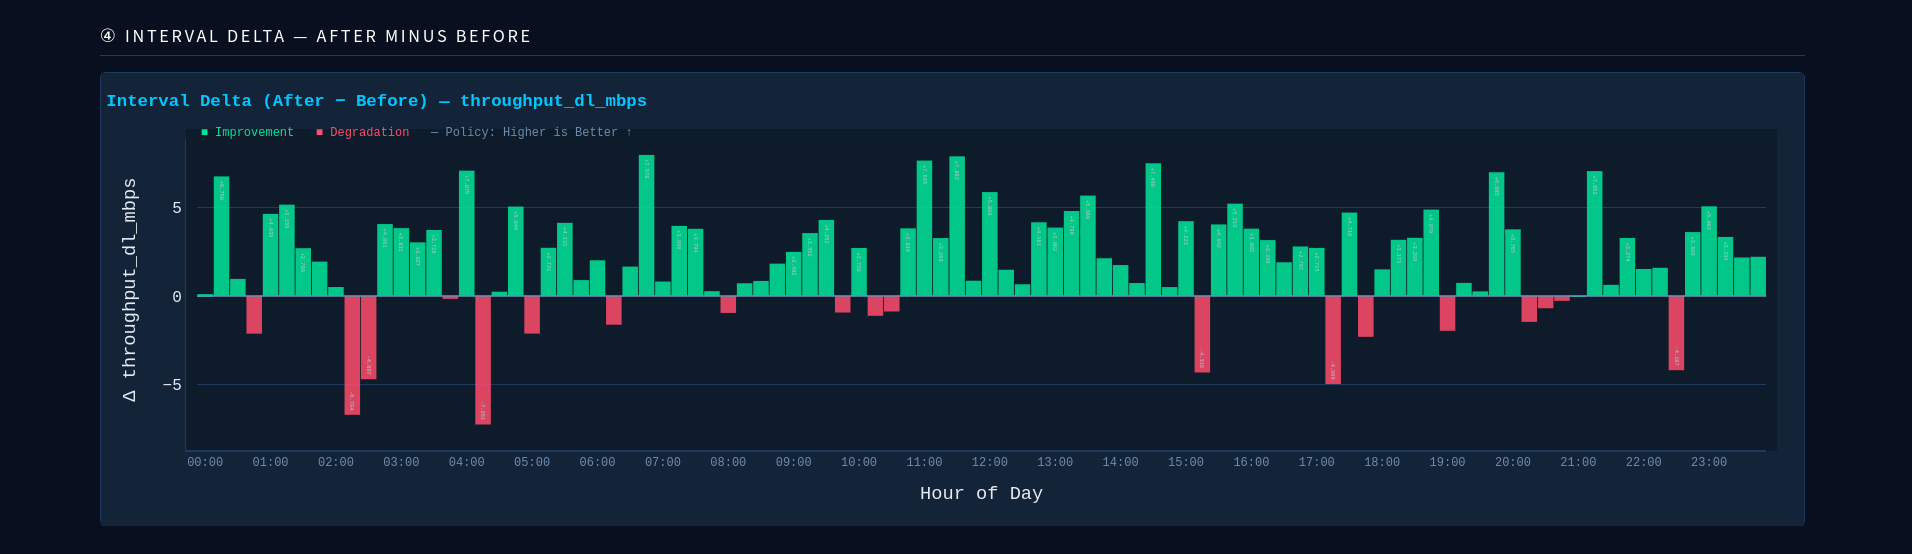
\includegraphics[width=0.85\textwidth]{delta_bars.png}
\end{frame}

\begin{frame}{KPI Impact Summary Table}
    \centering
    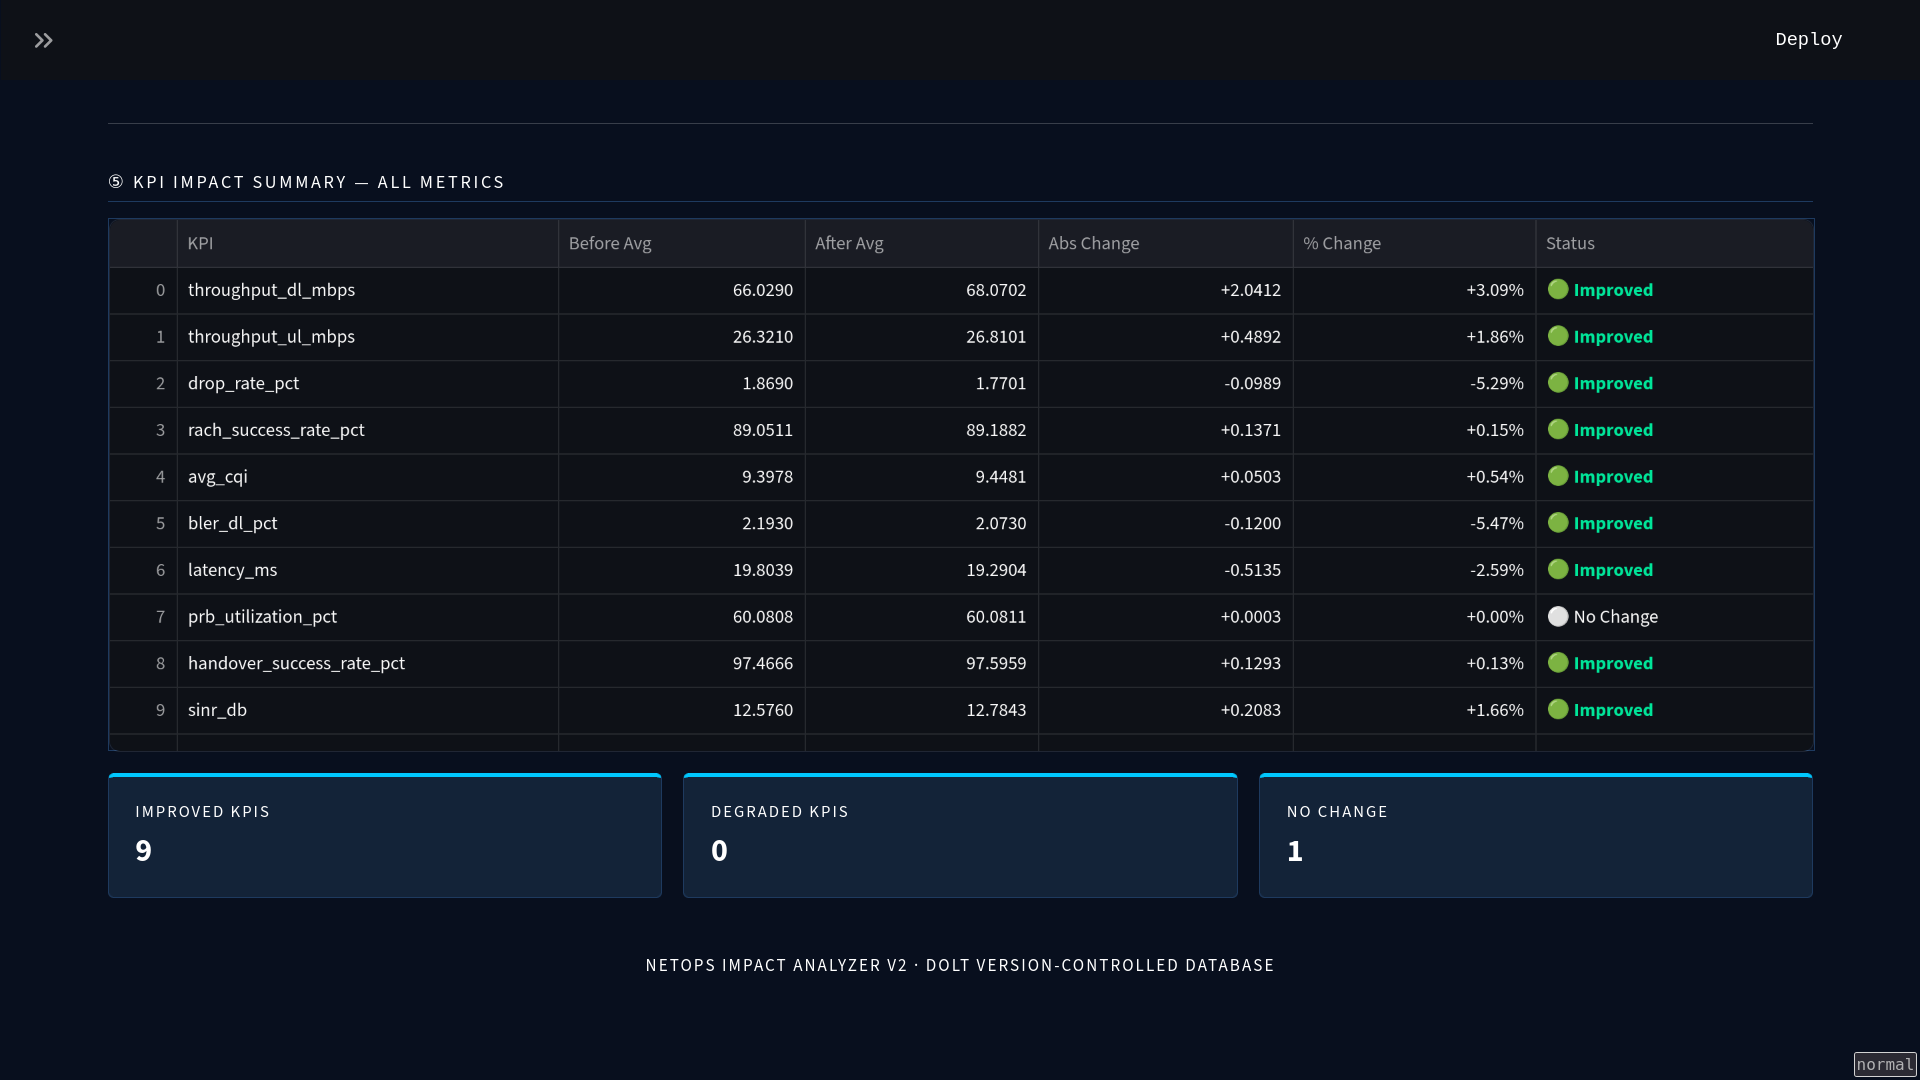
\includegraphics[width=0.85\textwidth]{summary_table.png}
\end{frame}

% ══════════════════════════════════════════════════════════
\section{User Workflow}

\begin{frame}{The Five-Step Analyst Workflow}
    \centering
    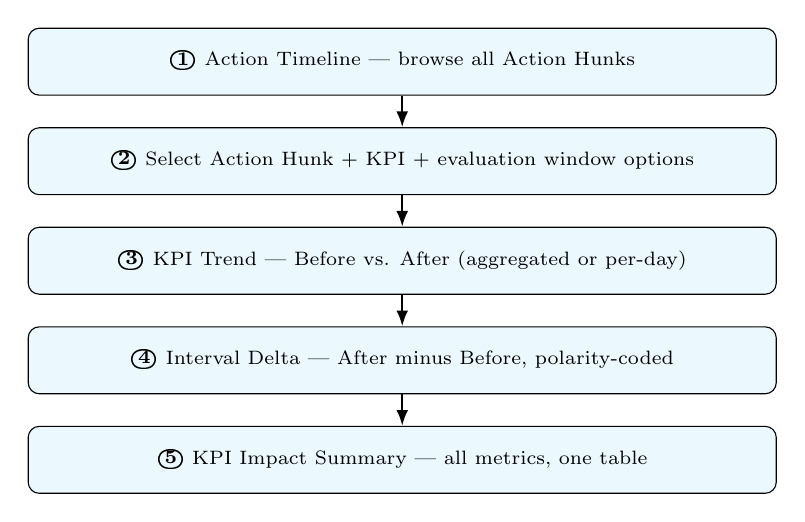
\begin{tikzpicture}[
        node distance=4mm,
        wstep/.style={draw, rounded corners, fill=cyan!8,
                     minimum width=9.5cm, minimum height=0.85cm,
                     align=left, font=\scriptsize},
        arrow/.style={-{Latex[length=2mm]}, thick}
    ]
        \node[wstep] (s1) {\textbf{\textcircled{1}} Action Timeline --- browse all Action Hunks};
        \node[wstep, below=of s1] (s2) {\textbf{\textcircled{2}} Select Action Hunk + KPI + evaluation window options};
        \node[wstep, below=of s2] (s3) {\textbf{\textcircled{3}} KPI Trend --- Before vs. After (aggregated or per-day)};
        \node[wstep, below=of s3] (s4) {\textbf{\textcircled{4}} Interval Delta --- After minus Before, polarity-coded};
        \node[wstep, below=of s4] (s5) {\textbf{\textcircled{5}} KPI Impact Summary --- all metrics, one table};
        \draw[arrow] (s1) -- (s2);
        \draw[arrow] (s2) -- (s3);
        \draw[arrow] (s3) -- (s4);
        \draw[arrow] (s4) -- (s5);
    \end{tikzpicture}

    \footnotesize The five-wstep analyst workflow implemented in
    \texttt{app.py}.
\end{frame}

\begin{frame}{Workflow Details}
    \small
    \begin{enumerate}
        \item \textbf{Action Timeline} --- visual context on all past
              optimization actions
        \item \textbf{Hunk \& Window Selection} --- metric tiles +
              expandable Dolt diff panel (table, column, from/to value)
        \item \textbf{KPI Trend} --- aggregated or per-weekday individual
              curves, with a time-of-day zoom slider
        \item \textbf{Interval Delta} --- polarity-coded magnitude of
              change per interval
        \item \textbf{Impact Summary} --- Improved/Degraded/No-Change
              verdict for every KPI at once
    \end{enumerate}
\end{frame}

% ══════════════════════════════════════════════════════════
\section{Technology Stack}

\begin{frame}{Technology Stack}
    \begin{tabular}{@{}ll@{}}
        \toprule
        \textbf{Layer} & \textbf{Technology} \\
        \midrule
        Database                  & Dolt (version-controlled MySQL-compatible) \\
        Database connector        & PyMySQL \\
        Data processing           & pandas, NumPy \\
        Visualization              & Plotly \\
        Web application / UI       & Streamlit \\
        Configuration persistence  & JSON (\texttt{kpi\_config.json}) \\
        \bottomrule
    \end{tabular}
\end{frame}

% ══════════════════════════════════════════════════════════
\section{Design Highlights}

\begin{frame}{Design Highlights}
    \begin{itemize}
        \item Version control \textbf{as} the audit trail
        \item Seasonality-aware statistics (weekday matching)
        \item Automatic evaluation-window boundary detection
        \item Zero-configuration KPI discovery
        \item Graceful degradation via mock-data mode
    \end{itemize}
\end{frame}


% ══════════════════════════════════════════════════════════
\section{Summary}

\begin{frame}{Summary}
    \begin{itemize}
        \item Pairs a version-controlled database with a
              seasonality-aware comparison engine and interactive
              visualization
        \item Turns manual, error-prone impact assessment into a
              repeatable, auditable, self-service tool
        \item Answers the central question: \emph{did this change
              actually help?}
    \end{itemize}
\end{frame}

\begin{frame}
    \centering
    \Huge  Questions?
   \vspace{1em}
  \end{frame}

\end{document}
